\documentclass[11pt,letterpaper]{article}
\usepackage[margin=1in]{geometry}
\usepackage{graphicx}
\usepackage{hyperref}
\usepackage{listings}
\usepackage{amsmath}
\pagestyle{headings}
\usepackage{epstopdf}

\begin{document}

\title{PHY 410 \\ Homework Assignment 8}
\author{Han Wen \\ \tiny Person No. 50096432}
\date{\today}

\maketitle

\begin{abstract}
The goal of this assignment is to get more familiar with RK-4 method in ODE, as well as other methods, examples of celestial orbits, quantum harmonic oscillator and Kronig-Penney model will be presented.  


\end{abstract}

\tableofcontents

\newpage
\section{Problem 1}

\subsection{Description}

Generate the orbits of (1) Halley's Comet and at least one planetary orbit using fixed-time step Runge-Kutta and adaptive time step Runge-Kutta and compare the efficiency of the two methods (you can estimate errors by measuring the period for example); and (2) a few interesting orbits near the Lagrangian points of the restricted 3-body problem, for example the Halo orbit selected by NASA for the James Webb telescope described by Dr. Mather earlier this year, or a Lissajous orbit.

\subsection{Numerical Analysis}

\subsubsection{part a}
Using the program, combined with the data from wikipedia ~\cite{Halley}, when using RK-4 method:
 Enter aphelion distance in AU: 35.1\\
 Enter eccentricity: 0.967\\
 Semimajor axis a =  17.8444331469  AU\\
 Period T =  75.3796531592  yr\\
 $v_y$(0) =  0.192656328719  AU/yr\\
 With the time step 0.001, the result is shown below: Fig. ~\ref{figure1}


\begin{figure}
\begin{center}
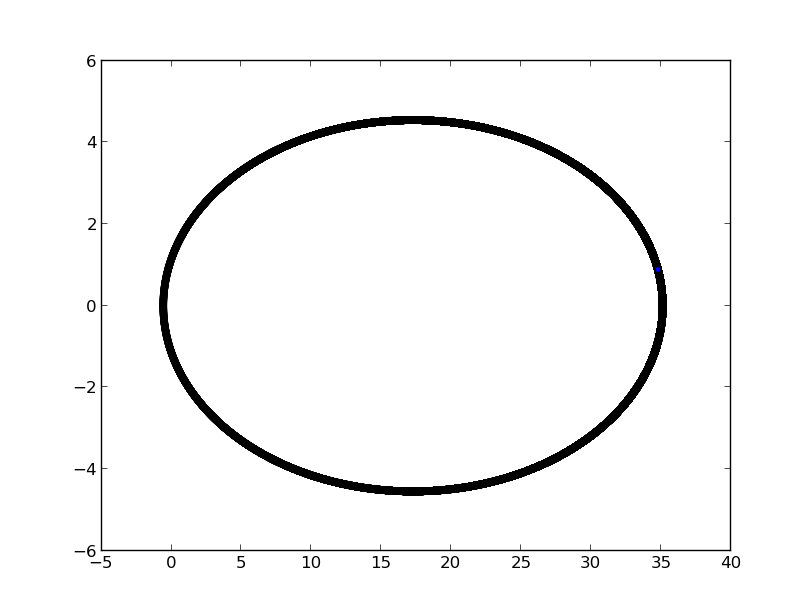
\includegraphics[width=0.8\linewidth,angle=0]{rk4.png}
\caption{Halley Comet orbit with RK4 method}
\label{figure1}
\end{center}
\end{figure}

When using RK-4 adaptive method:
 Enter aphelion distance in AU: 35.1\\
 Enter eccentricity: 0.967\\
 Semimajor axis a =  17.8444331469  AU\\
 Period T =  75.3796531592  yr\\
 $v_y$(0) =  0.192656328719  AU/yr\\
 Enter step size dt: 0.001\\
 Enter desired accuracy for adaptive integration: 0.000001\\
 The result is shown below: Fig ~\ref{figure2}

\begin{figure}
\begin{center}
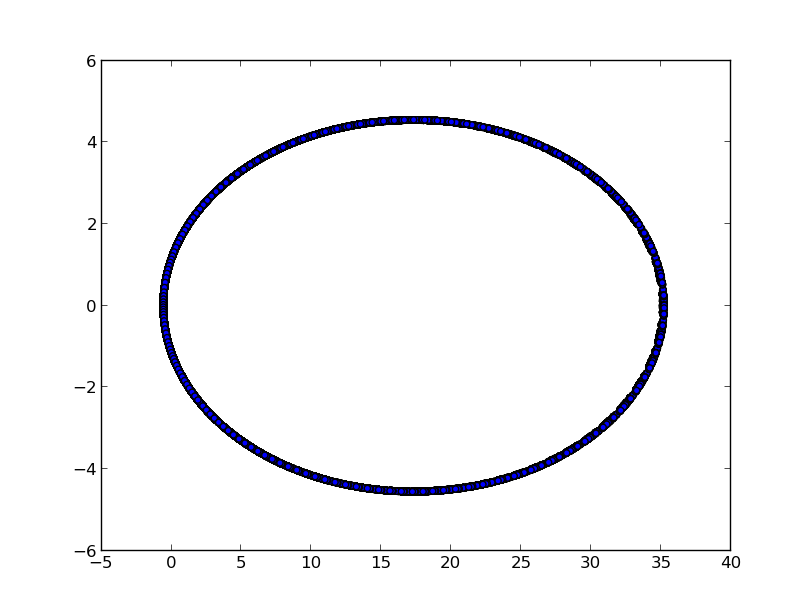
\includegraphics[width=0.8\linewidth,angle=0]{rk4ad.png}
\caption{Halley Comet orbit with RK4-adaptive method}
\label{figure2}
\end{center}
\end{figure}

I found in this case the regular RK-4 method is more efficient.

\subsubsection{part b}

With the parameters included in here ~\cite{Lpoint}, around point L2, with the proper initial condition, I generate the halo orbit shown here: Fig. ~\ref{figure3}. We can see it's fairly a good plot, although since the data is not precise enough, a little "Lissajous orbit" style will be mixed into the simulation plot.

\begin{figure}
\begin{center}
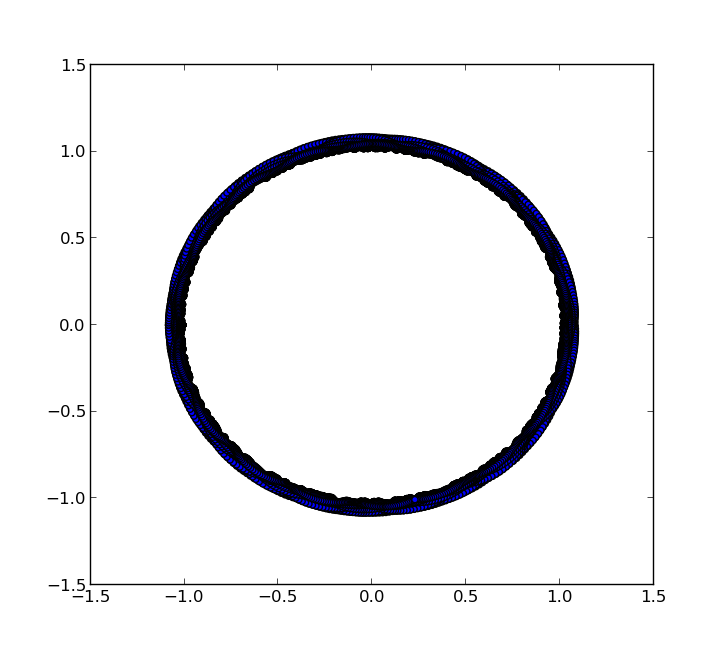
\includegraphics[width=0.8\linewidth,angle=0]{halo.png}
\caption{Halo orbit}
\label{figure3}
\end{center}
\end{figure}

\newpage

\section{Problem 2}

\subsection{Description}
Modify the Schroedinger code to add (1) a cubic $x^3$ term and (2) a quartic $x^4$ term, to the harmonic oscillator potential. Discuss how each type of perturbation modifies the energy levels and eigenfunctions. Be sure to increase the left and right boundaries if needed! 


\subsection{Result}

To be consistent with the perturbation theory, I added a parameter $\lambda$ before the cubic or the quartic term, and making $\lambda$ a rather small number. I chose E=5 in our case so that the number of eigenvalues is appropriate.
Without the perturbation, the result is: 
 Level       Energy           Simple Steps   Secant Steps\\
 -----   ------------------   ------------   ------------\\
   -1.001250     0.500076\\
    1.001250     0.500076\\
\\
   -1.732500     1.500095\\
    1.732500     1.500095\\
\\
   -2.236250     2.500113\\
    2.236250     2.500113\\
\\
   -2.646250     3.500115\\
    2.646250     3.500115\\
\\
   -3.001250     4.500120\\
    3.001250     4.500120\\
\\
   -3.317500     5.500139\\
    3.317500     5.500139\\
With the diagram: Fig ~\ref{figure4}


\begin{figure}
\begin{center}
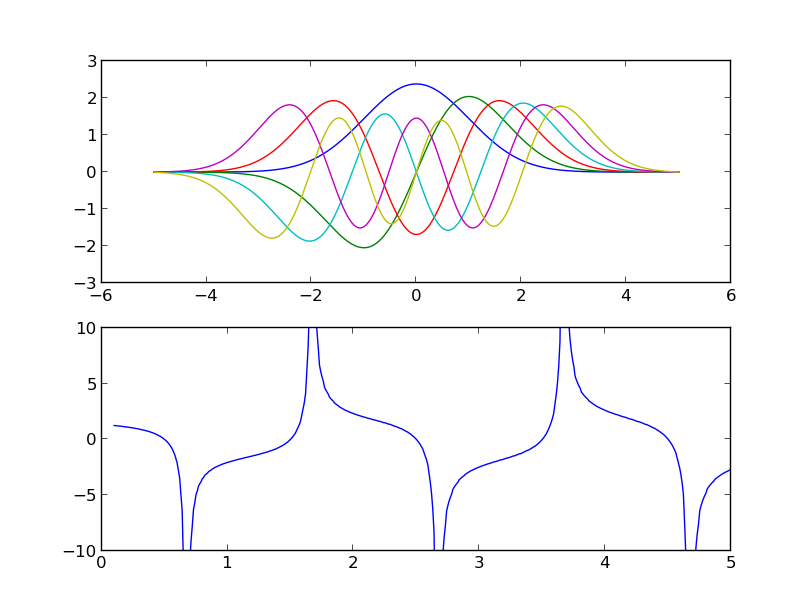
\includegraphics[width=0.8\linewidth,angle=0]{p2origin.png}
\caption{Harmonic oscillation without perturbation}
\label{figure4}
\end{center}
\end{figure}

When it comes to cubic perturbation, with $\lambda=0.05$:

 Level       Energy           Simple Steps   Secant Steps\\
 -----   ------------------   ------------   ------------\\
   -9.903750     0.475473\\
    0.933750     0.475473\\
\\
   -9.697500     1.422769\\
    1.568750     1.422769\\
\\
   -9.482500     2.329516\\
    1.973750     2.329516\\
\\
   -9.262500     3.166497\\
    2.272500     3.166497\\
\\
   -9.041250     3.921575\\
    2.505000     3.921575\\
\\
   -8.811250     4.618098\\
    2.697500     4.618098\\
\\
   -8.198750     6.054249\\
    3.047500     6.054249\\

And the plot: ~\ref{figure5}

\begin{figure}
\begin{center}
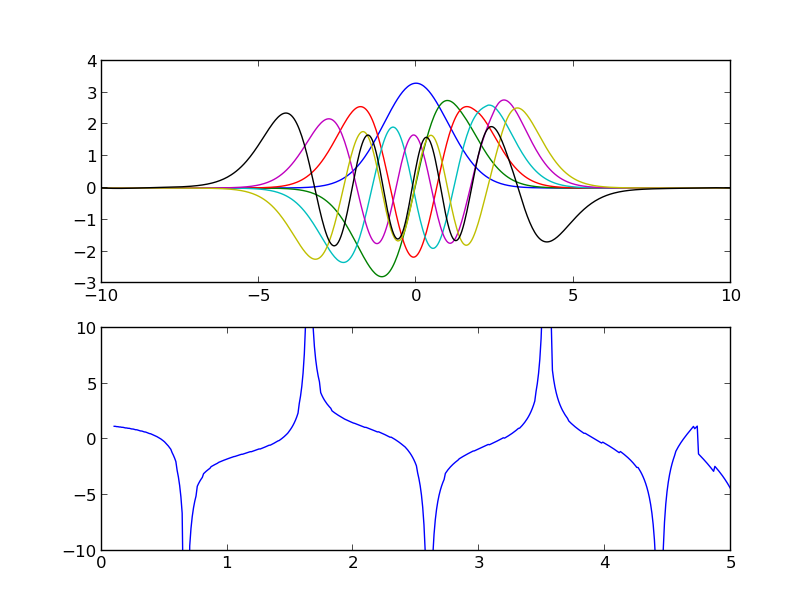
\includegraphics[width=0.8\linewidth,angle=0]{p2x3.png}
\caption{Harmonic oscillation with cubic perturbation}
\label{figure5}
\end{center}
\end{figure}

When quadric perturbation, with $\lambda=0.05$:

 Level       Energy           Simple Steps   Secant Steps\\
 -----   ------------------   ------------   ------------\\
   -0.986250     0.532749\\
    0.986250     0.532749\\
\\
   -1.620000     1.653598\\
    1.620000     1.653598\\
\\
   -2.021250     2.874194\\
    2.021250     2.874194\\
\\
   -2.328750     4.176595\\
    2.328750     4.176595\\
\\
   -2.581250     5.549612\\
    2.581250     5.549612\\

And the plot: ~\ref{figure6}

\begin{figure}
\begin{center}
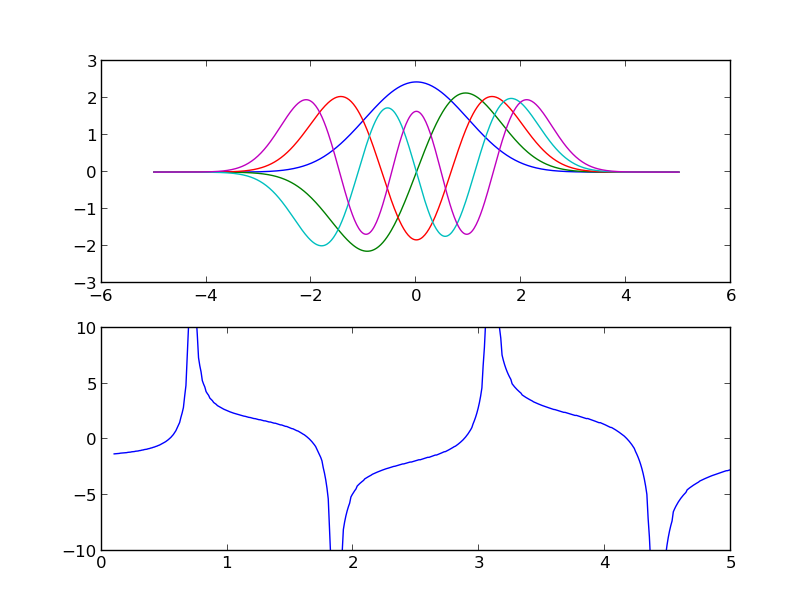
\includegraphics[width=0.8\linewidth,angle=0]{p2x4.png}
\caption{Harmonic oscillation with quadric perturbation}
\label{figure6}
\end{center}
\end{figure}
\newpage

We can see, with the cubic perturbation, the number of energy level increase from 5 to 6, the whole numbers of level shifted and the values of energy for the first 5 levels decrease a little, while with the quadric perturbation, the number remains the same and the values of energy increase a little. Those property origin from the form of the perturbation, namely the cubic form is antisymmetric and the quadric one is symmetric.




  
\section{Problem 3}
\subsection{Description}
Study the dependence of the Kronig-Penney model band structure on the width and height of the potential step, and describe any systematic trends you notice.


\subsection{Result}

Guided by the theoretical result as well as the symmetric property of the system. Based on the result of different trials, I found when fix the width and increase the height, the band gap increase Fig ~\ref{figure7}. When fix the the height and change the width, the more close the width is to half of the size of the unit cell, the bigger the gap. When the width is approaching 0 or the size of the unit cell, the gap is vanishing. ~\ref{figure8} 



\begin{figure}
\begin{center}
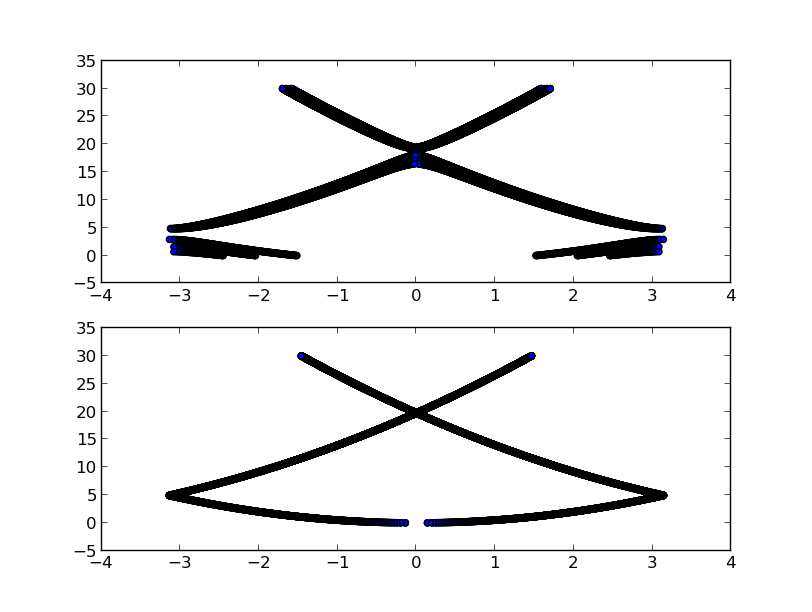
\includegraphics[width=0.8\linewidth,angle=0]{kp.png}
\caption{Kronig Penney with height -5 -8 -10 and width 0.2}
\label{figure7}
\end{center}
\end{figure}

\begin{figure}
\begin{center}
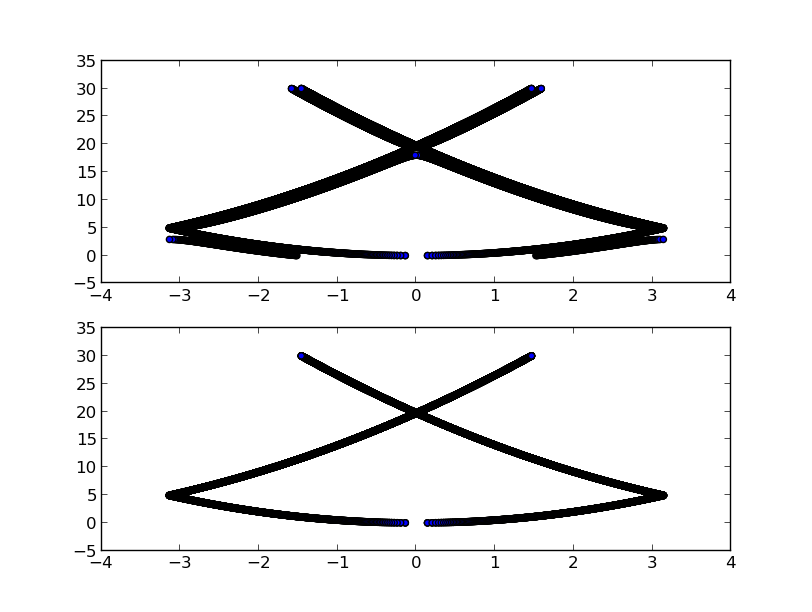
\includegraphics[width=0.8\linewidth,angle=0]{kpw.png}
\caption{Kronig Penney with width 0.2 0.5 1.0 and height -5.0}
\label{figure8}
\end{center}
\end{figure}

Here is the plot with width 0.2 height -5.0 Fig ~\ref{figure9}

\begin{figure}
\begin{center}
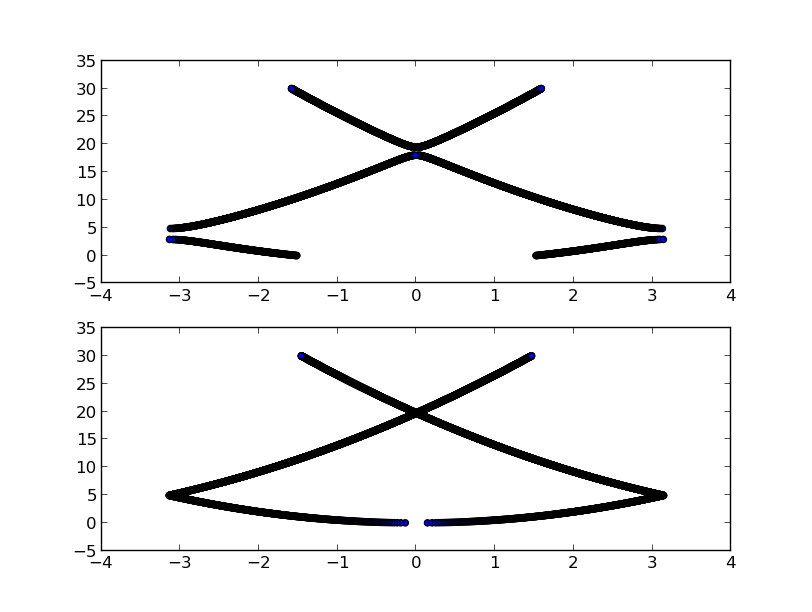
\includegraphics[width=0.8\linewidth,angle=0]{kp0250.png}
\caption{Kronig Penney with width 0.2 height -5.0}
\label{figure9}
\end{center}
\end{figure}



Here is the plot with width 0.5 height -5.0 Fig ~\ref{figure10}

\begin{figure}
\begin{center}
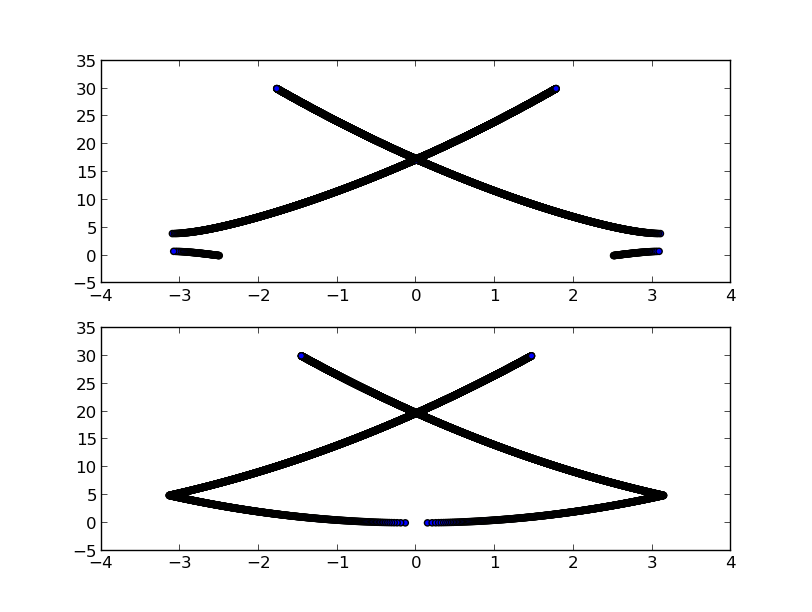
\includegraphics[width=0.8\linewidth,angle=0]{kp0550.png}
\caption{Kronig Penney with width 0.5 height -5.0}
\label{figure10}
\end{center}
\end{figure}


Here is the plot with width 0.2 height -10.0 Fig ~\ref{figure11}


\begin{figure}
\begin{center}
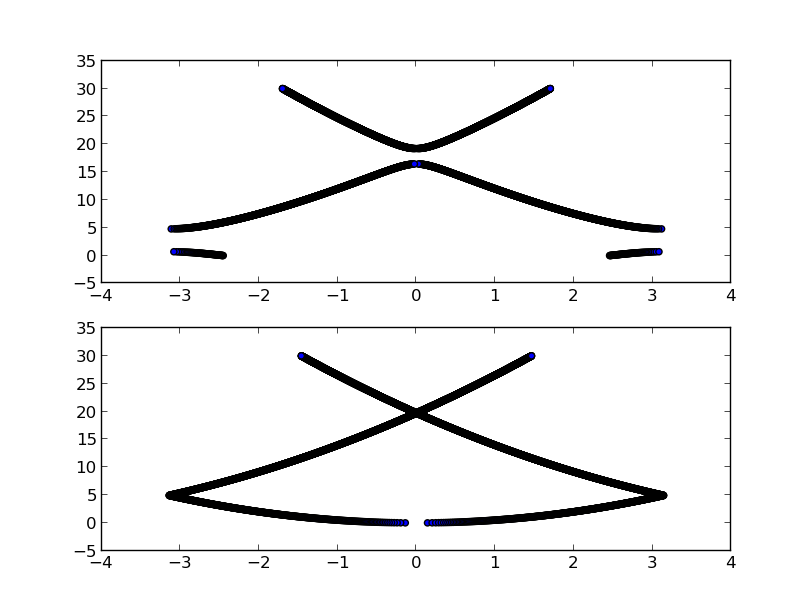
\includegraphics[width=0.8\linewidth,angle=0]{kp0210.png}
\caption{Kronig Penney with width 0.2 height -10.0}
\label{figure11}
\end{center}
\end{figure}


\newpage
\section*{Acknowledgements}

I discussed this assignment with my classmates and used material from the
cited references, but this write-up is my own.

\begin{thebibliography}{9}


\bibitem{coursepage}
PHY 410-505 Webpage, \url{http://www.physics.buffalo.edu/phy410-505}.



\bibitem{Halley}
Halley Comet Wikipedia 
\url{http://en.wikipedia.org/wiki/Halley%27s_Comet}

\bibitem{Lpoint}
Lagrange point
\url{http://www.physics.montana.edu/faculty/cornish/lagrange.pdf}

\end{thebibliography}

\newpage
\appendix
\section{Appendix}

\subsection{python code}

The following python code was used to obtain the results in this report:

\lstinputlisting[language=python]{kepler.py}

\lstinputlisting[language=python]{rcp3body.py}

\lstinputlisting[language=python]{schroedinger.py}

\lstinputlisting[language=python]{kronig_penneywh.py}

\end{document}
